\subsection{Proposal}
\label{subsec:proposal}
In general there exists some characteristics, in the vehicles, we are looking for:
a) Provenance,
b) Transparency with respects to purchase sale,
c) Traceability with history transactions, owners and legal situations (including  
government participation).

To achieve these goals, we have proposed a distributed model illustrated in the context
diagram in Figure~\ref{fig:flowChartFramework}. Such a figure denotes
the general stages (circled numbers) a user must follow to get or set information about a 
vehicle:
\begin{figure}[hb]
 %\begin{center}
  \centering
    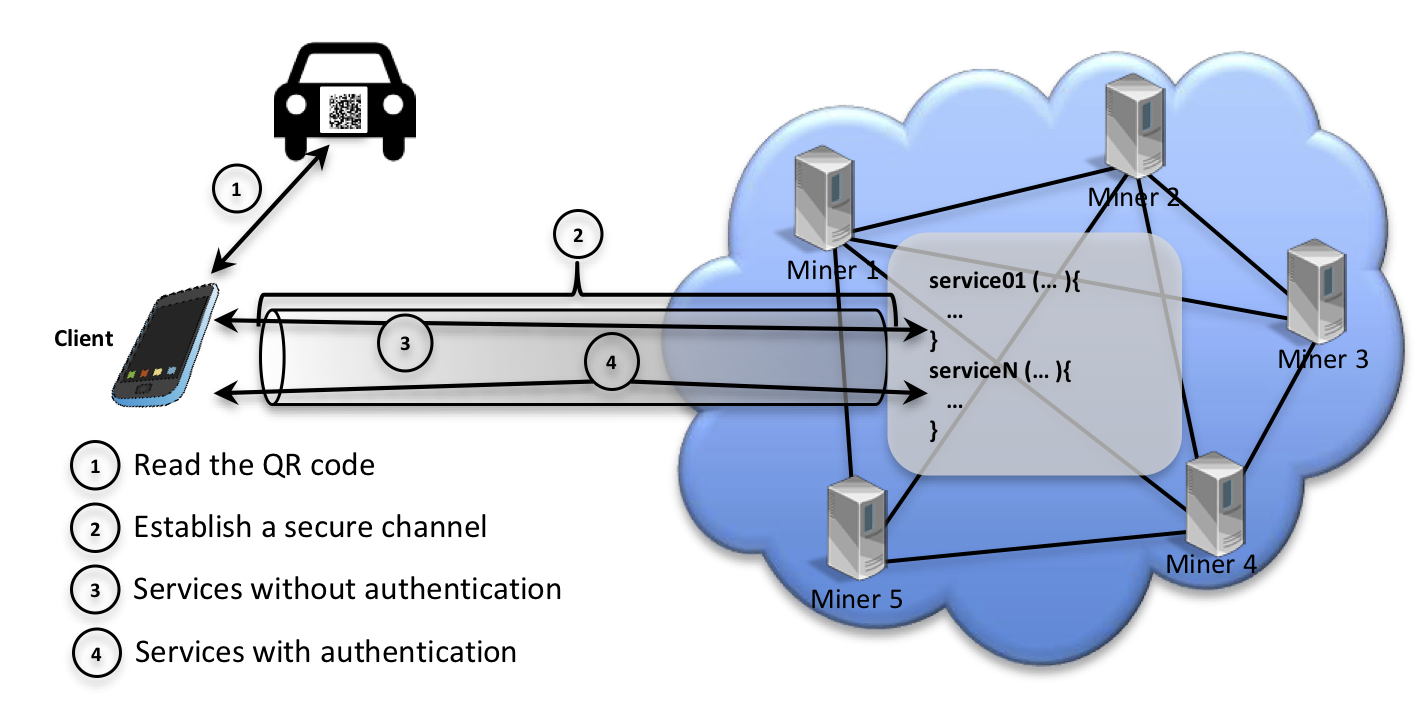
\includegraphics[scale=0.74]{images/lopez2.png}
        \caption{Diagram about the use of the framework from the client view}
    \label{fig:flowChartFramework}
 % \end{center}
\end{figure}

\begin{itemize}
  \item \textbf{Stage I} consists in getting information of a vehicle through reading
    a QR code by any user.
    %or setting the QR code by a dealership. 
    This stage requires that a company generates the genesis block after a vehicle has 
    been manufactured. Details in Section~\ref{ssec:clientServer}.
  \item \textbf{Stage II} consists in establishing a secure channel between any user
    and the \textit{vehicle blockchain network}. We
    have used the TLS protocol because it is the standard in the
    e-commerce and it has been subject to a lot of verification proofs.
    Details in Section~\ref{sec:secureChannel}.
  \item \textbf{Stage III} consists in getting services such as provenance or 
    traceability. Some services require authentication, but others do not.
    Details in Section~\ref{sec:getServices}.  
  \item \textbf{Stage IV:} consists in how to do transactions and what kind of these can 
    do each role (owner, government, dealerships, etc). For example how to build
    the genesis block within the \textit{vehicle blockchain network}. 
    Authentication is required. 
    Details in Section~\ref{sec:transactions}. 
\end{itemize}

\subsection{Notation}
\label{sec:notation}
%As you can see, our stages imply the use of cryptography,  and security protocol techniques. 
% The following two sub-sections describe the notation used in the rest of
% the document. 

% \subsubsection{Host level notation}
% \label{sec:hostLevel}
Our notation has some similarities with Burrows et.al.~\cite{Burrows1990}. 
Table~\ref{table:conventions} summarizes our notation. Let start with
cryptography, it has two main mechanisms:
\begin{itemize}
  \item Symmetric cryptography, the same key is used to encode and
    decode a message; by convention, symbol $\fat{m}_{K_{AB}}$ will be
    used to denote that a message $m$ has been cyphered under the key
    $K_{AB}$, which agents $A$ and $B$ know. \footnote{An agent is a 
        computer process that uses the client-server technology to 
        establish a network communication. Sometimes we will use the 
        terms agent or client indistinctly.} 
  \item Asymmetric cryptography, two keys are used to encode and
    decode messages; an agent (e.g. $A$) has a key pair
    (public $K_{pub(A)}$ and private $K_{priv(A)}$). One key used to
    encode and the other one to decode (reciprocally); usually, key
    $K_{priv(A)}$ is kept in secret. 
\end{itemize}

\begin{table}[htb]
\footnotesize
\begin{center}
\caption{Conventions in types of messages and agents}
\label{table:conventions}
\begin{tabular}{|l|l|}
\hline
{\bf Abbreviation}& {\bf Description}                                   \\\hline\hline
$C$                 &  Agent, Client or Smartphone application able to \\
                    &  establish communication with other agent.         \\ 
$\Server$           &  A trusted agent, best known as trusted Miner-Server      \\
$K$                 &  Symmetric key                                      \\
$K_{AB}$            &  Symmetric key shared with agents $A$ and $B$       \\
$K_{pub(A)}$        &  Public key of Agent $A$                            \\
$K_{priv(A)}$       &  Private key of Agent $A$                           \\
$\fat{m}_{K}$       &  Message $m$ cyphered under key $K$                 \\
$m1\lnk m2$         &  $m1$ and $m2$ are concatenated using symbol $\lnk$ \\
$[m_1:: m_2]$       &  A list o messages, $m_1$ representing the first element\\
$N_a$, $N_b$, $N_c$ &  Nonces, which are random unguessable numbers      \\
                    &  never been used before.                           \\ \hline \hline
\end{tabular}
\end{center}
\end{table}
\normalsize

% \subsubsection{Notation at network level}
% \label{sec:networkLevel}
Table~\ref{table:NetConventions} describes the notation in the Client-Server communication.
Our model is compound by various security protocols. A security protocol is formed by the 
initial knowledge of the participant agents and a set of message steps. Each step consists in  
sending or receiving messages under the Client-Server technology. Before sending a message,
an agent can execute an operation (maybe dependent of the previous received message), as part 
of a local process.

%three views (see ): i) initial knowledge;
%ii) message sending and message reception; and iii) the local process
%representation.
\begin{table}[htb]
\footnotesize
\begin{center}
\caption{Conventions in network level}
\label{table:NetConventions}
\begin{tabular}{|l|l|}
\hline
{\bf Abbreviation}                      & {\bf Description}                    \\\hline\hline
\textbf{Initial knowledge:}             &                                      \\
$A : ik$                                &  Initially agent $A$ knows $ik$.    \\ \hline 
\textbf{Message Sending and Receiving:} &  At step $n$ agent $A$ sends         \\ 
$n. A \rightarrow B: m$                 &  message $m$ to agent $B$,\\
                                        &  which $B$ receives.      \\ \hline 
$n. A\rightarrow B: m$                  &  message $m2$ was generated \\ 
\hspace{5mm}\textbf{Local process:}     &  Between steps $n$ and $n2$,    \\ 
\hspace{5mm}$m2 = f(m)$                 &  by $B$ as a local process \\ 
$n2. B\rightarrow A: m2$                &  generated from $f(m)$.     \\ \hline 
\textbf{Broadcast:}                     &  $A$ broadcasts message to agents\\ 
$A \rightarrow [B, C, D]: m$            &  $B$, $C$ and $D$.\\ \hline \hline 
\end{tabular}
\end{center}
\end{table}
\normalsize


$$$$

